% Options for packages loaded elsewhere
\PassOptionsToPackage{unicode}{hyperref}
\PassOptionsToPackage{hyphens}{url}
%
\documentclass[
  ignorenonframetext,
]{beamer}
\usepackage{pgfpages}
\setbeamertemplate{caption}[numbered]
\setbeamertemplate{caption label separator}{: }
\setbeamercolor{caption name}{fg=normal text.fg}
\beamertemplatenavigationsymbolsempty
% Prevent slide breaks in the middle of a paragraph
\widowpenalties 1 10000
\raggedbottom
\setbeamertemplate{part page}{
  \centering
  \begin{beamercolorbox}[sep=16pt,center]{part title}
    \usebeamerfont{part title}\insertpart\par
  \end{beamercolorbox}
}
\setbeamertemplate{section page}{
  \centering
  \begin{beamercolorbox}[sep=12pt,center]{part title}
    \usebeamerfont{section title}\insertsection\par
  \end{beamercolorbox}
}
\setbeamertemplate{subsection page}{
  \centering
  \begin{beamercolorbox}[sep=8pt,center]{part title}
    \usebeamerfont{subsection title}\insertsubsection\par
  \end{beamercolorbox}
}
\AtBeginPart{
  \frame{\partpage}
}
\AtBeginSection{
  \ifbibliography
  \else
    \frame{\sectionpage}
  \fi
}
\AtBeginSubsection{
  \frame{\subsectionpage}
}
\usepackage{amsmath,amssymb}
\usepackage{iftex}
\ifPDFTeX
  \usepackage[T1]{fontenc}
  \usepackage[utf8]{inputenc}
  \usepackage{textcomp} % provide euro and other symbols
\else % if luatex or xetex
  \usepackage{unicode-math} % this also loads fontspec
  \defaultfontfeatures{Scale=MatchLowercase}
  \defaultfontfeatures[\rmfamily]{Ligatures=TeX,Scale=1}
\fi
\usepackage{lmodern}
\usetheme[]{Singapore}
\ifPDFTeX\else
  % xetex/luatex font selection
\fi
% Use upquote if available, for straight quotes in verbatim environments
\IfFileExists{upquote.sty}{\usepackage{upquote}}{}
\IfFileExists{microtype.sty}{% use microtype if available
  \usepackage[]{microtype}
  \UseMicrotypeSet[protrusion]{basicmath} % disable protrusion for tt fonts
}{}
\makeatletter
\@ifundefined{KOMAClassName}{% if non-KOMA class
  \IfFileExists{parskip.sty}{%
    \usepackage{parskip}
  }{% else
    \setlength{\parindent}{0pt}
    \setlength{\parskip}{6pt plus 2pt minus 1pt}}
}{% if KOMA class
  \KOMAoptions{parskip=half}}
\makeatother
\usepackage{xcolor}
\newif\ifbibliography
\usepackage{graphicx}
\makeatletter
\def\maxwidth{\ifdim\Gin@nat@width>\linewidth\linewidth\else\Gin@nat@width\fi}
\def\maxheight{\ifdim\Gin@nat@height>\textheight\textheight\else\Gin@nat@height\fi}
\makeatother
% Scale images if necessary, so that they will not overflow the page
% margins by default, and it is still possible to overwrite the defaults
% using explicit options in \includegraphics[width, height, ...]{}
\setkeys{Gin}{width=\maxwidth,height=\maxheight,keepaspectratio}
% Set default figure placement to htbp
\makeatletter
\def\fps@figure{htbp}
\makeatother
\setlength{\emergencystretch}{3em} % prevent overfull lines
\providecommand{\tightlist}{%
  \setlength{\itemsep}{0pt}\setlength{\parskip}{0pt}}
\setcounter{secnumdepth}{-\maxdimen} % remove section numbering
% definitions for citeproc citations
\NewDocumentCommand\citeproctext{}{}
\NewDocumentCommand\citeproc{mm}{%
  \begingroup\def\citeproctext{#2}\cite{#1}\endgroup}
\makeatletter
 % allow citations to break across lines
 \let\@cite@ofmt\@firstofone
 % avoid brackets around text for \cite:
 \def\@biblabel#1{}
 \def\@cite#1#2{{#1\if@tempswa , #2\fi}}
\makeatother
\newlength{\cslhangindent}
\setlength{\cslhangindent}{1.5em}
\newlength{\csllabelwidth}
\setlength{\csllabelwidth}{3em}
\newenvironment{CSLReferences}[2] % #1 hanging-indent, #2 entry-spacing
 {\begin{list}{}{%
  \setlength{\itemindent}{0pt}
  \setlength{\leftmargin}{0pt}
  \setlength{\parsep}{0pt}
  % turn on hanging indent if param 1 is 1
  \ifodd #1
   \setlength{\leftmargin}{\cslhangindent}
   \setlength{\itemindent}{-1\cslhangindent}
  \fi
  % set entry spacing
  \setlength{\itemsep}{#2\baselineskip}}}
 {\end{list}}
\usepackage{calc}
\newcommand{\CSLBlock}[1]{\hfill\break\parbox[t]{\linewidth}{\strut\ignorespaces#1\strut}}
\newcommand{\CSLLeftMargin}[1]{\parbox[t]{\csllabelwidth}{\strut#1\strut}}
\newcommand{\CSLRightInline}[1]{\parbox[t]{\linewidth - \csllabelwidth}{\strut#1\strut}}
\newcommand{\CSLIndent}[1]{\hspace{\cslhangindent}#1}
\AtBeginSection[]{}
\usepackage{graphicx}
\logo{\ifnum\thepage>1
\includegraphics[width=2cm]{Imagem1.jpg}\fi}
\titlegraphic{
\includegraphics[width=3cm]{Imagem1.jpg}}
\ifLuaTeX
  \usepackage{selnolig}  % disable illegal ligatures
\fi
\usepackage{bookmark}
\IfFileExists{xurl.sty}{\usepackage{xurl}}{} % add URL line breaks if available
\urlstyle{same}
\hypersetup{
  pdftitle={State policy vs.~Government policy},
  pdfauthor={Vinícius Pinon},
  hidelinks,
  pdfcreator={LaTeX via pandoc}}

\title{State policy vs.~Government policy}
\subtitle{How does political balance affect public policy approval?}
\author{Vinícius Pinon}
\date{2024-12-11}

\begin{document}
\frame{\titlepage}

\section{Motivation}\label{motivation}

\begin{frame}{Motivation}
\phantomsection\label{motivation-1}
\begin{figure}
\centering

\includegraphics[width=0.8\textwidth,height=\textheight]{programas.png}
\caption{Brazil and Mexico}
\end{figure}

\begin{itemize}
\tightlist
\item
  Strictness in policy design and implementation \footnotesize (De La O,
  2013)\normalsize;
\item
  Temptation to politicize in a polarized scenario;
\item
  The political ``balance'' \footnotesize Abramovay and Lotta,
  2022\normalsize.
\end{itemize}
\end{frame}

\begin{frame}{Summary}
\phantomsection\label{summary}
\begin{itemize}
\tightlist
\item
  RQ: Does political balance affect the approval of public policies?
\item
  Objectives
\end{itemize}

\begin{enumerate}
[1)]
\tightlist
\item
  Mapping the relationship between ownership and institutionalization;
\item
  Analyzing the effects of partisanship on policy approval;
\item
  Evaluating how institutionalization shapes public opinion.
\end{enumerate}
\end{frame}

\section{Theory and hypotheses}\label{theory-and-hypotheses}

\begin{frame}{The politics of policies}
\phantomsection\label{the-politics-of-policies}
\begin{itemize}
\tightlist
\item
  The power of partisanship (Abramowitz and Webster 2018);
\item
  From ``issue ownership'' to policy ownership (Petrocik 1996);
\item
  Politicization? Not always.
\end{itemize}

\begin{figure}
\centering
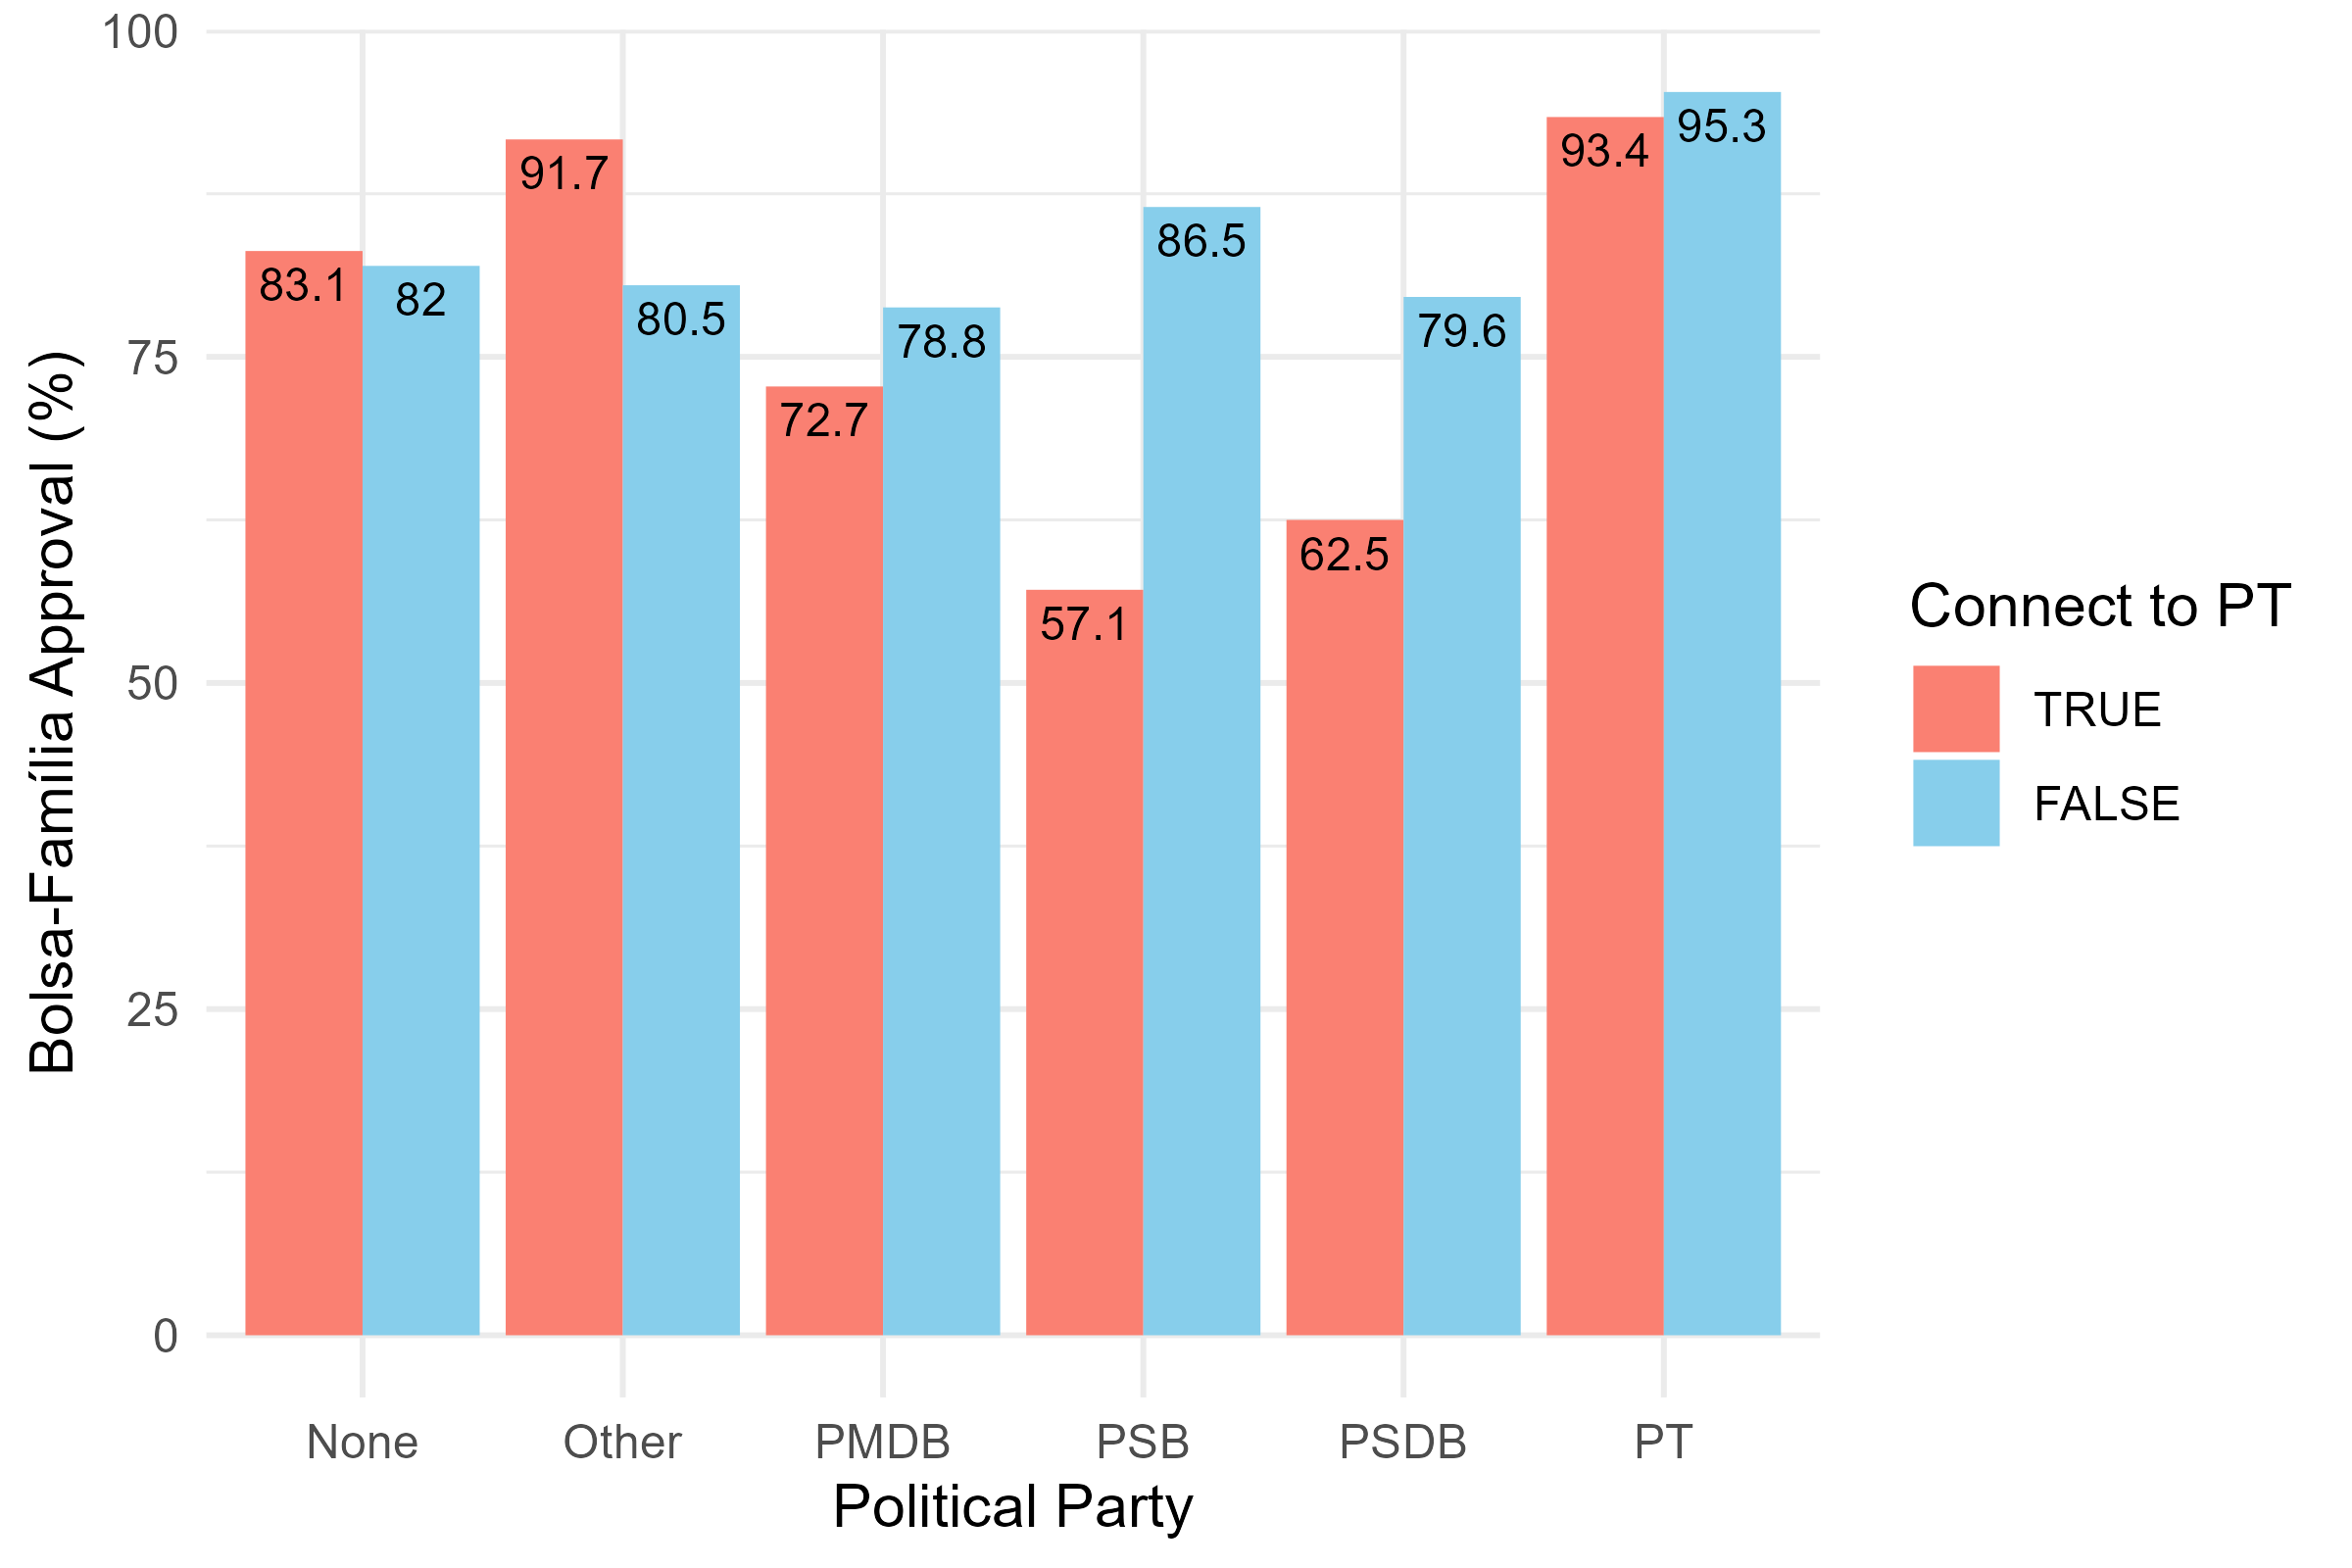
\includegraphics[width=0.55\textwidth,height=\textheight]{plots/figure_beps.png}
\caption{Mean PBF Approval by Party}
\end{figure}
\end{frame}

\begin{frame}{The institutionalization of policies}
\phantomsection\label{the-institutionalization-of-policies}
\begin{figure}
\centering
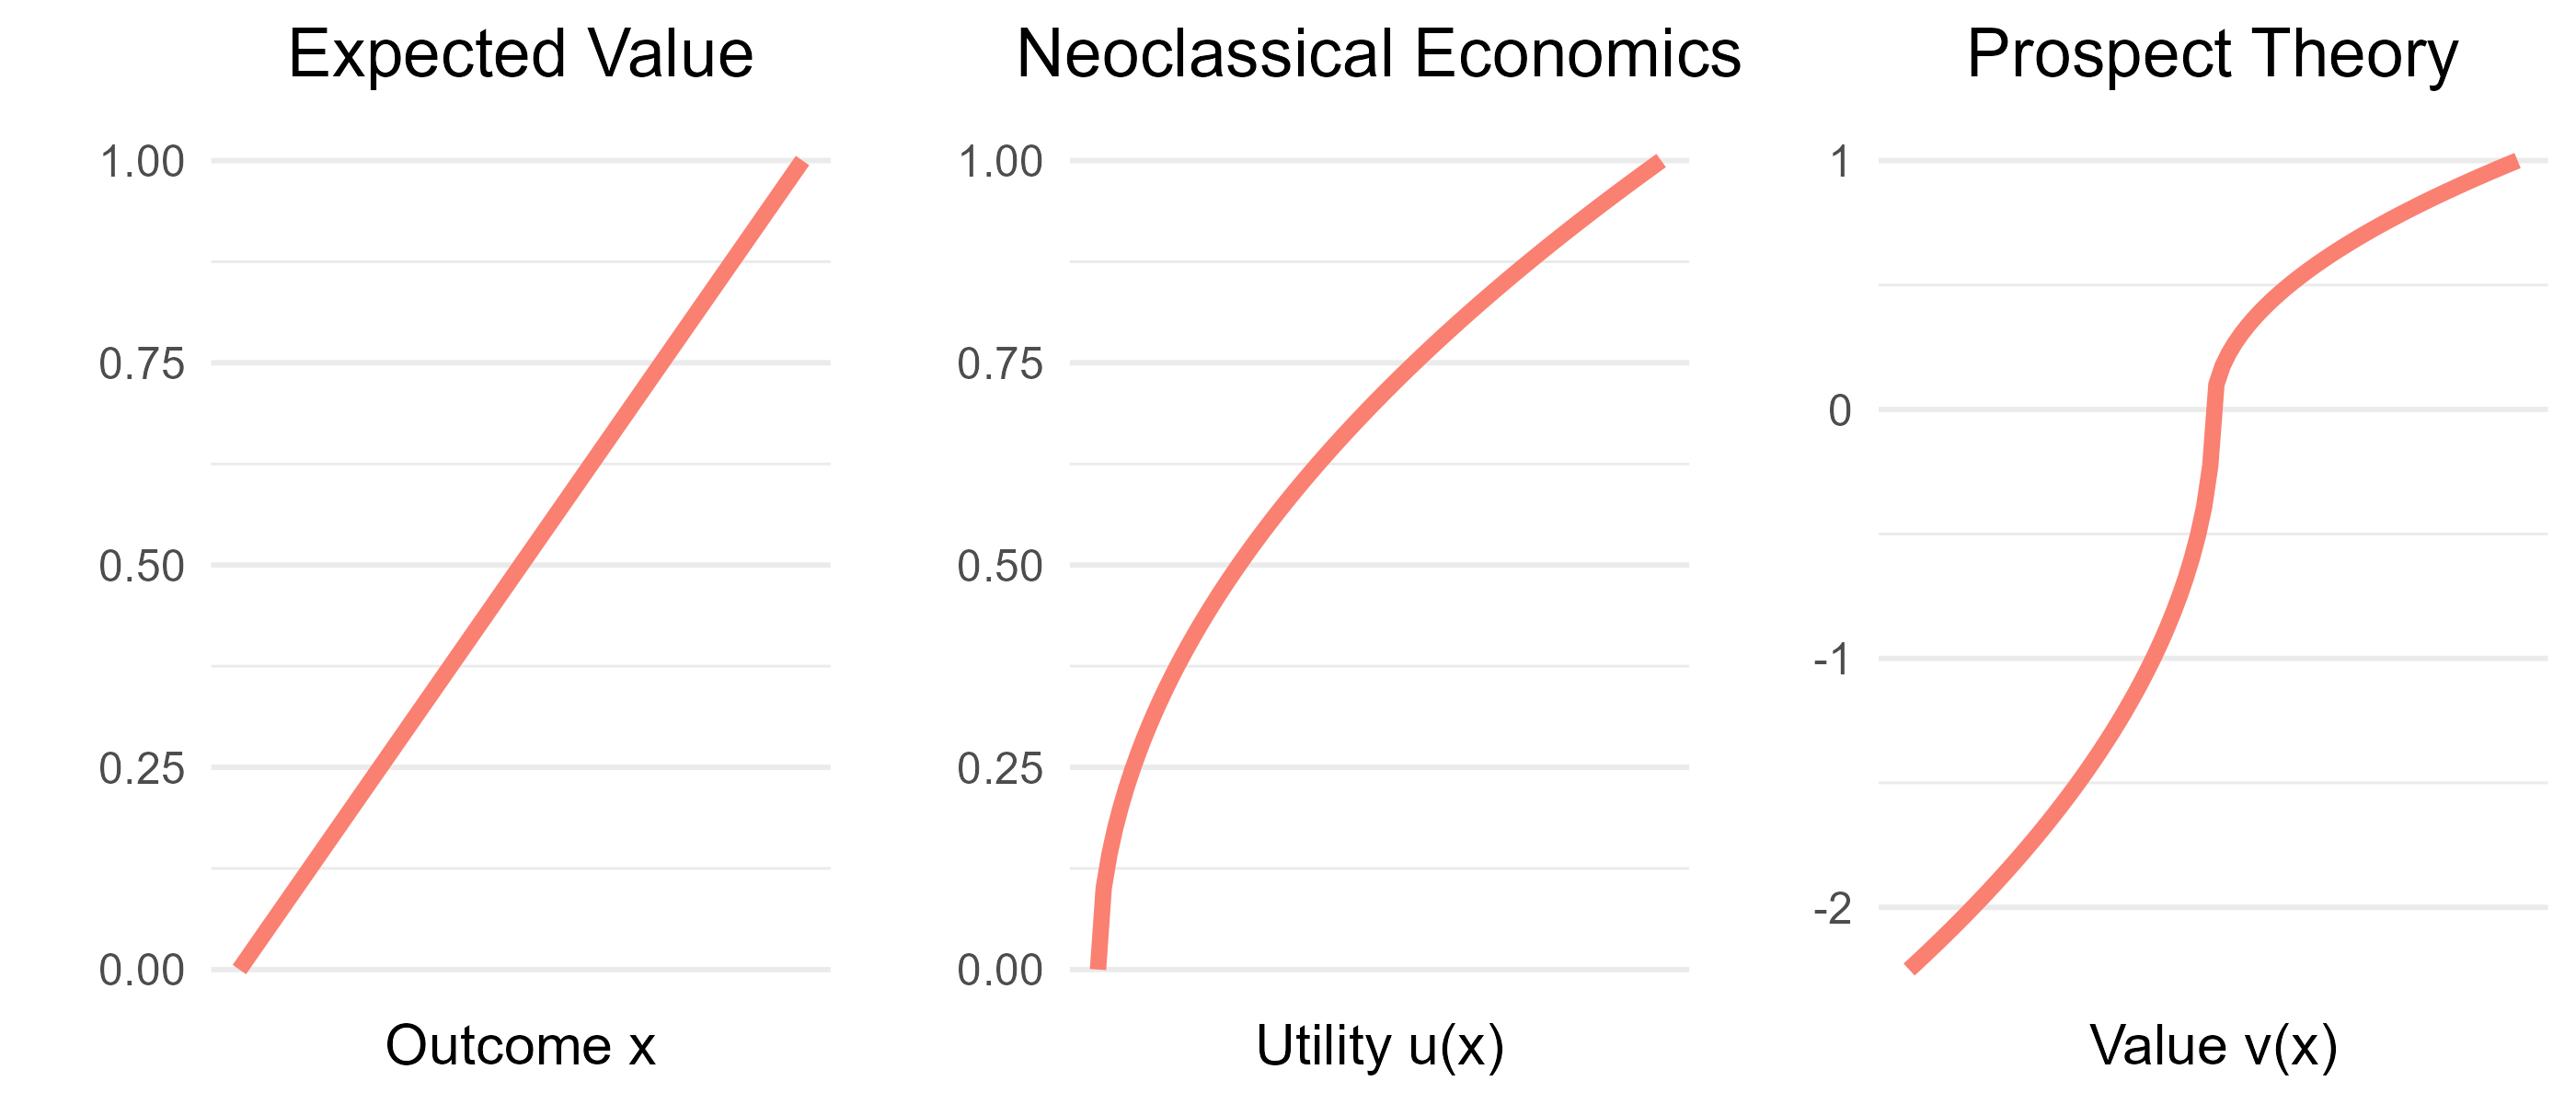
\includegraphics[width=0.6\textwidth,height=\textheight]{plots/figure_utility.png}
\caption{Main Utility Functions}
\end{figure}

\begin{itemize}
\tightlist
\item
  The rules (North 1990) and their entrenchment (Levitsky and Murillo
  2009);
\item
  Policy feedback literature;
\item
  Non-Politicization? Not always;
\item
  Status quo bias and loss aversion (Kahneman and Tversky 1979).
\end{itemize}
\end{frame}

\begin{frame}{Hypotheses}
\phantomsection\label{hypotheses}
\begin{itemize}
\tightlist
\item
  H1: Institutionalization is not associated with policy ownership;
\item
  H2a: Alignment with the policy owner positively affects policy
  approval;
\item
  H2b: Misalignment with the policy owner negatively affects policy
  approval;
\item
  H2c: Policy ownership negatively affects non-partisans' policy
  approval;
\item
  H3: Institutionalization positively affects the policy approval.
\end{itemize}
\end{frame}

\section{Empirical strategy}\label{empirical-strategy}

\begin{frame}{Empirical strategy}
\begin{itemize}
\tightlist
\item
  Choice-based conjoint experiment (Hainmueller, Hopkins, and Yamamoto
  2014);
\item
  Two surveys:
\end{itemize}

\begin{enumerate}
[1)]
\tightlist
\item
  Conjoint (N = 245)
\item
  Conjoint + Questions about real policies (N = 285)
\end{enumerate}
\end{frame}

\begin{frame}{Study 1}
\phantomsection\label{study-1}
\begin{figure}
\centering

\includegraphics[width=0.6\textwidth,height=\textheight]{plots/figure_amce.png}
\caption{Conjoint AMCE}
\end{figure}
\end{frame}

\begin{frame}{Study 2}
\phantomsection\label{study-2}
\begin{figure}
\centering
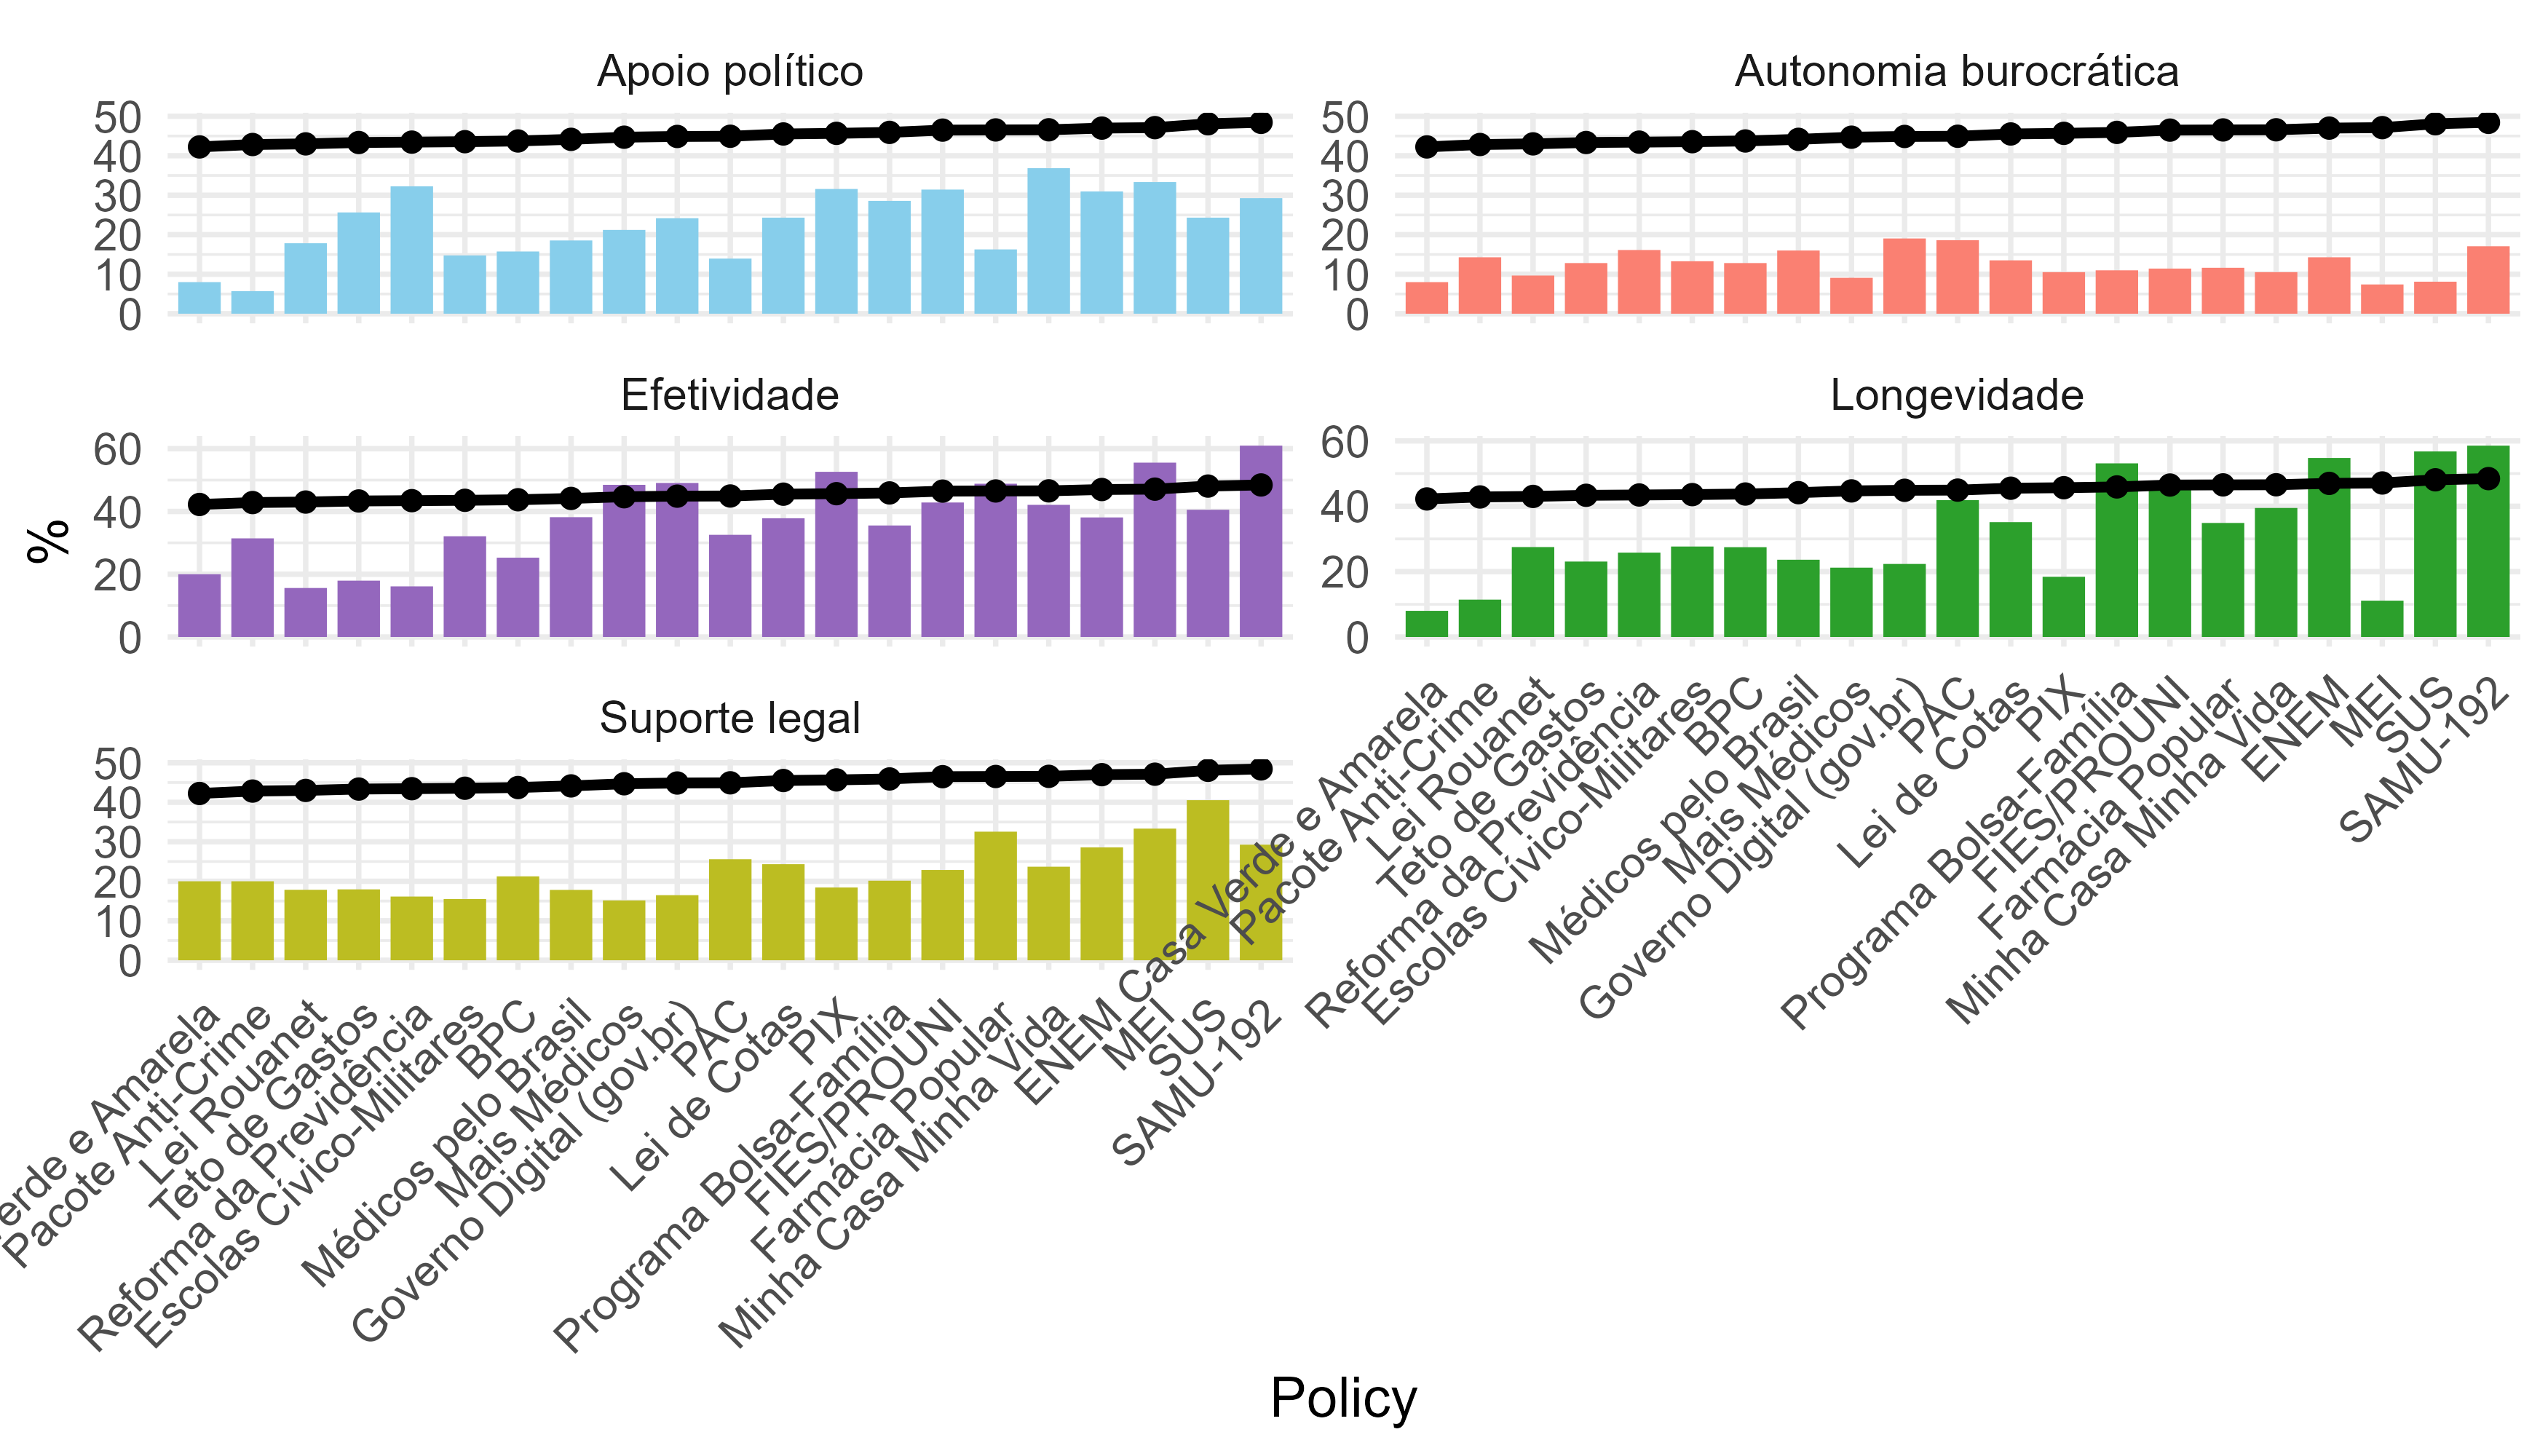
\includegraphics[width=0.7\textwidth,height=\textheight]{plots/figure_attributes.png}
\caption{Perceived attributes of the policies}
\end{figure}
\end{frame}

\begin{frame}{Study 3}
\phantomsection\label{study-3}
\begin{figure}
\centering
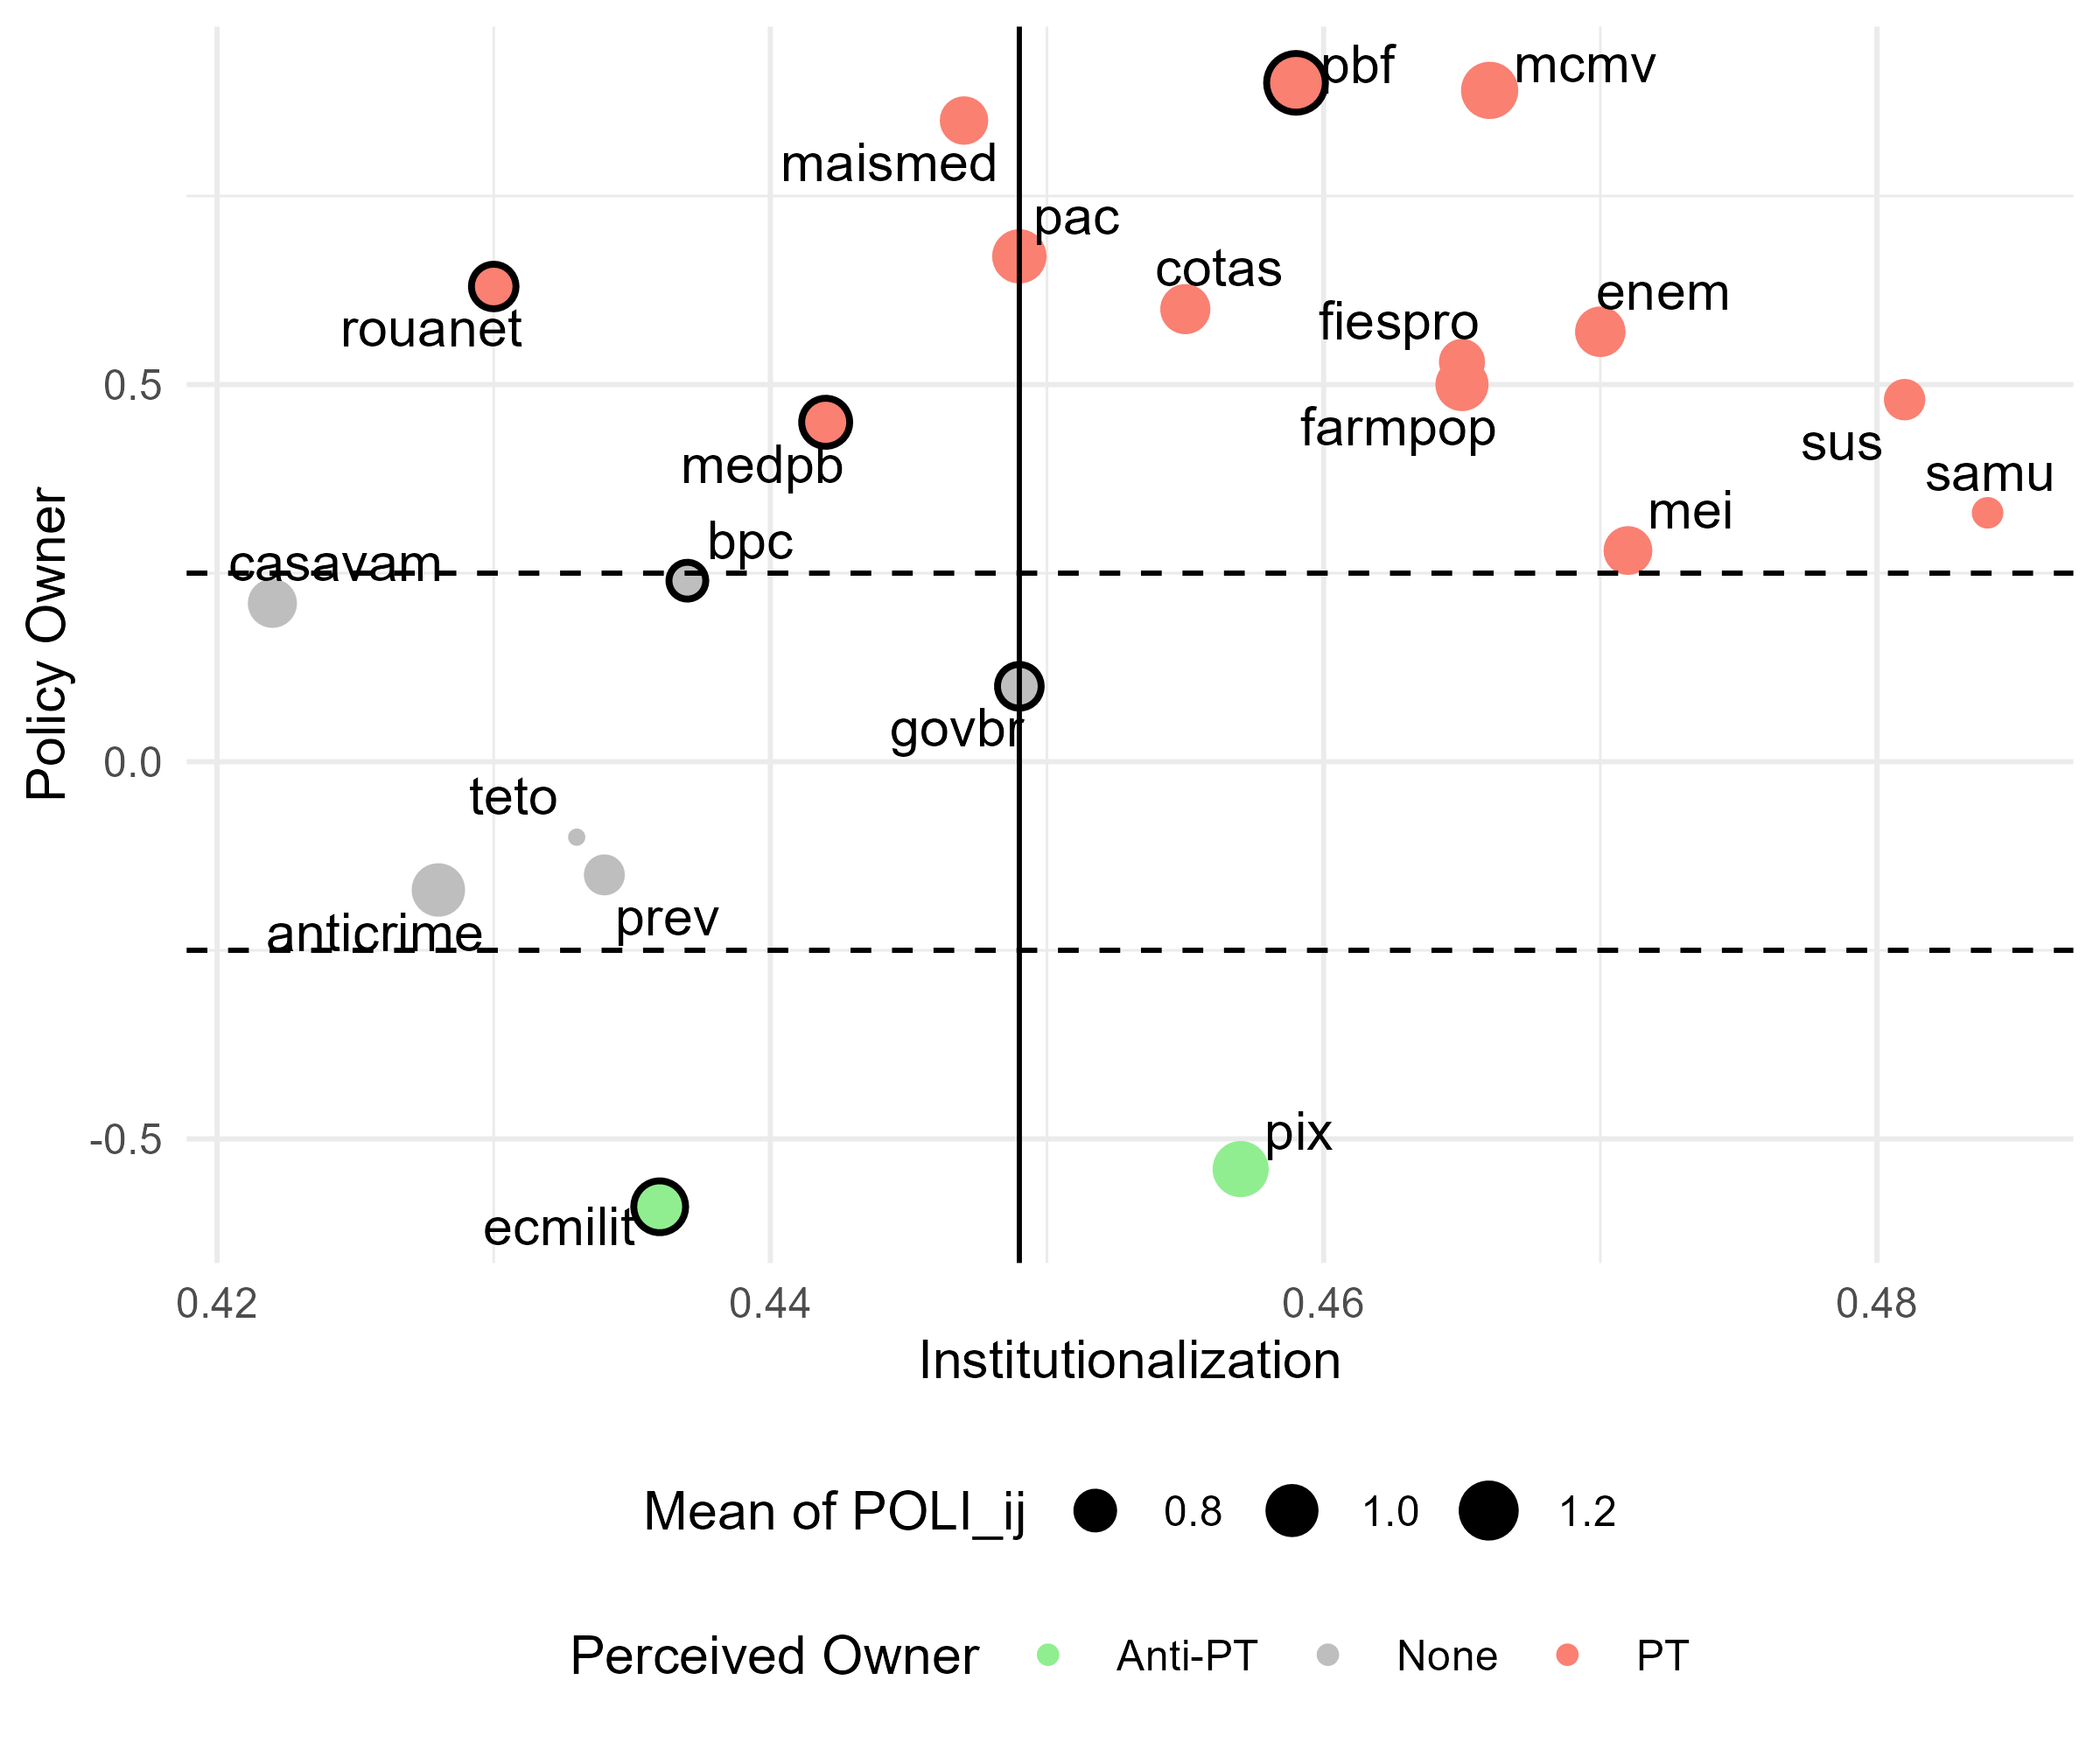
\includegraphics[width=0.55\textwidth,height=\textheight]{plots/figure_quadrante.png}
\caption{2x3 Summary}
\end{figure}
\end{frame}

\begin{frame}{Study 3}
\phantomsection\label{study-3-1}
\begin{figure}
\centering
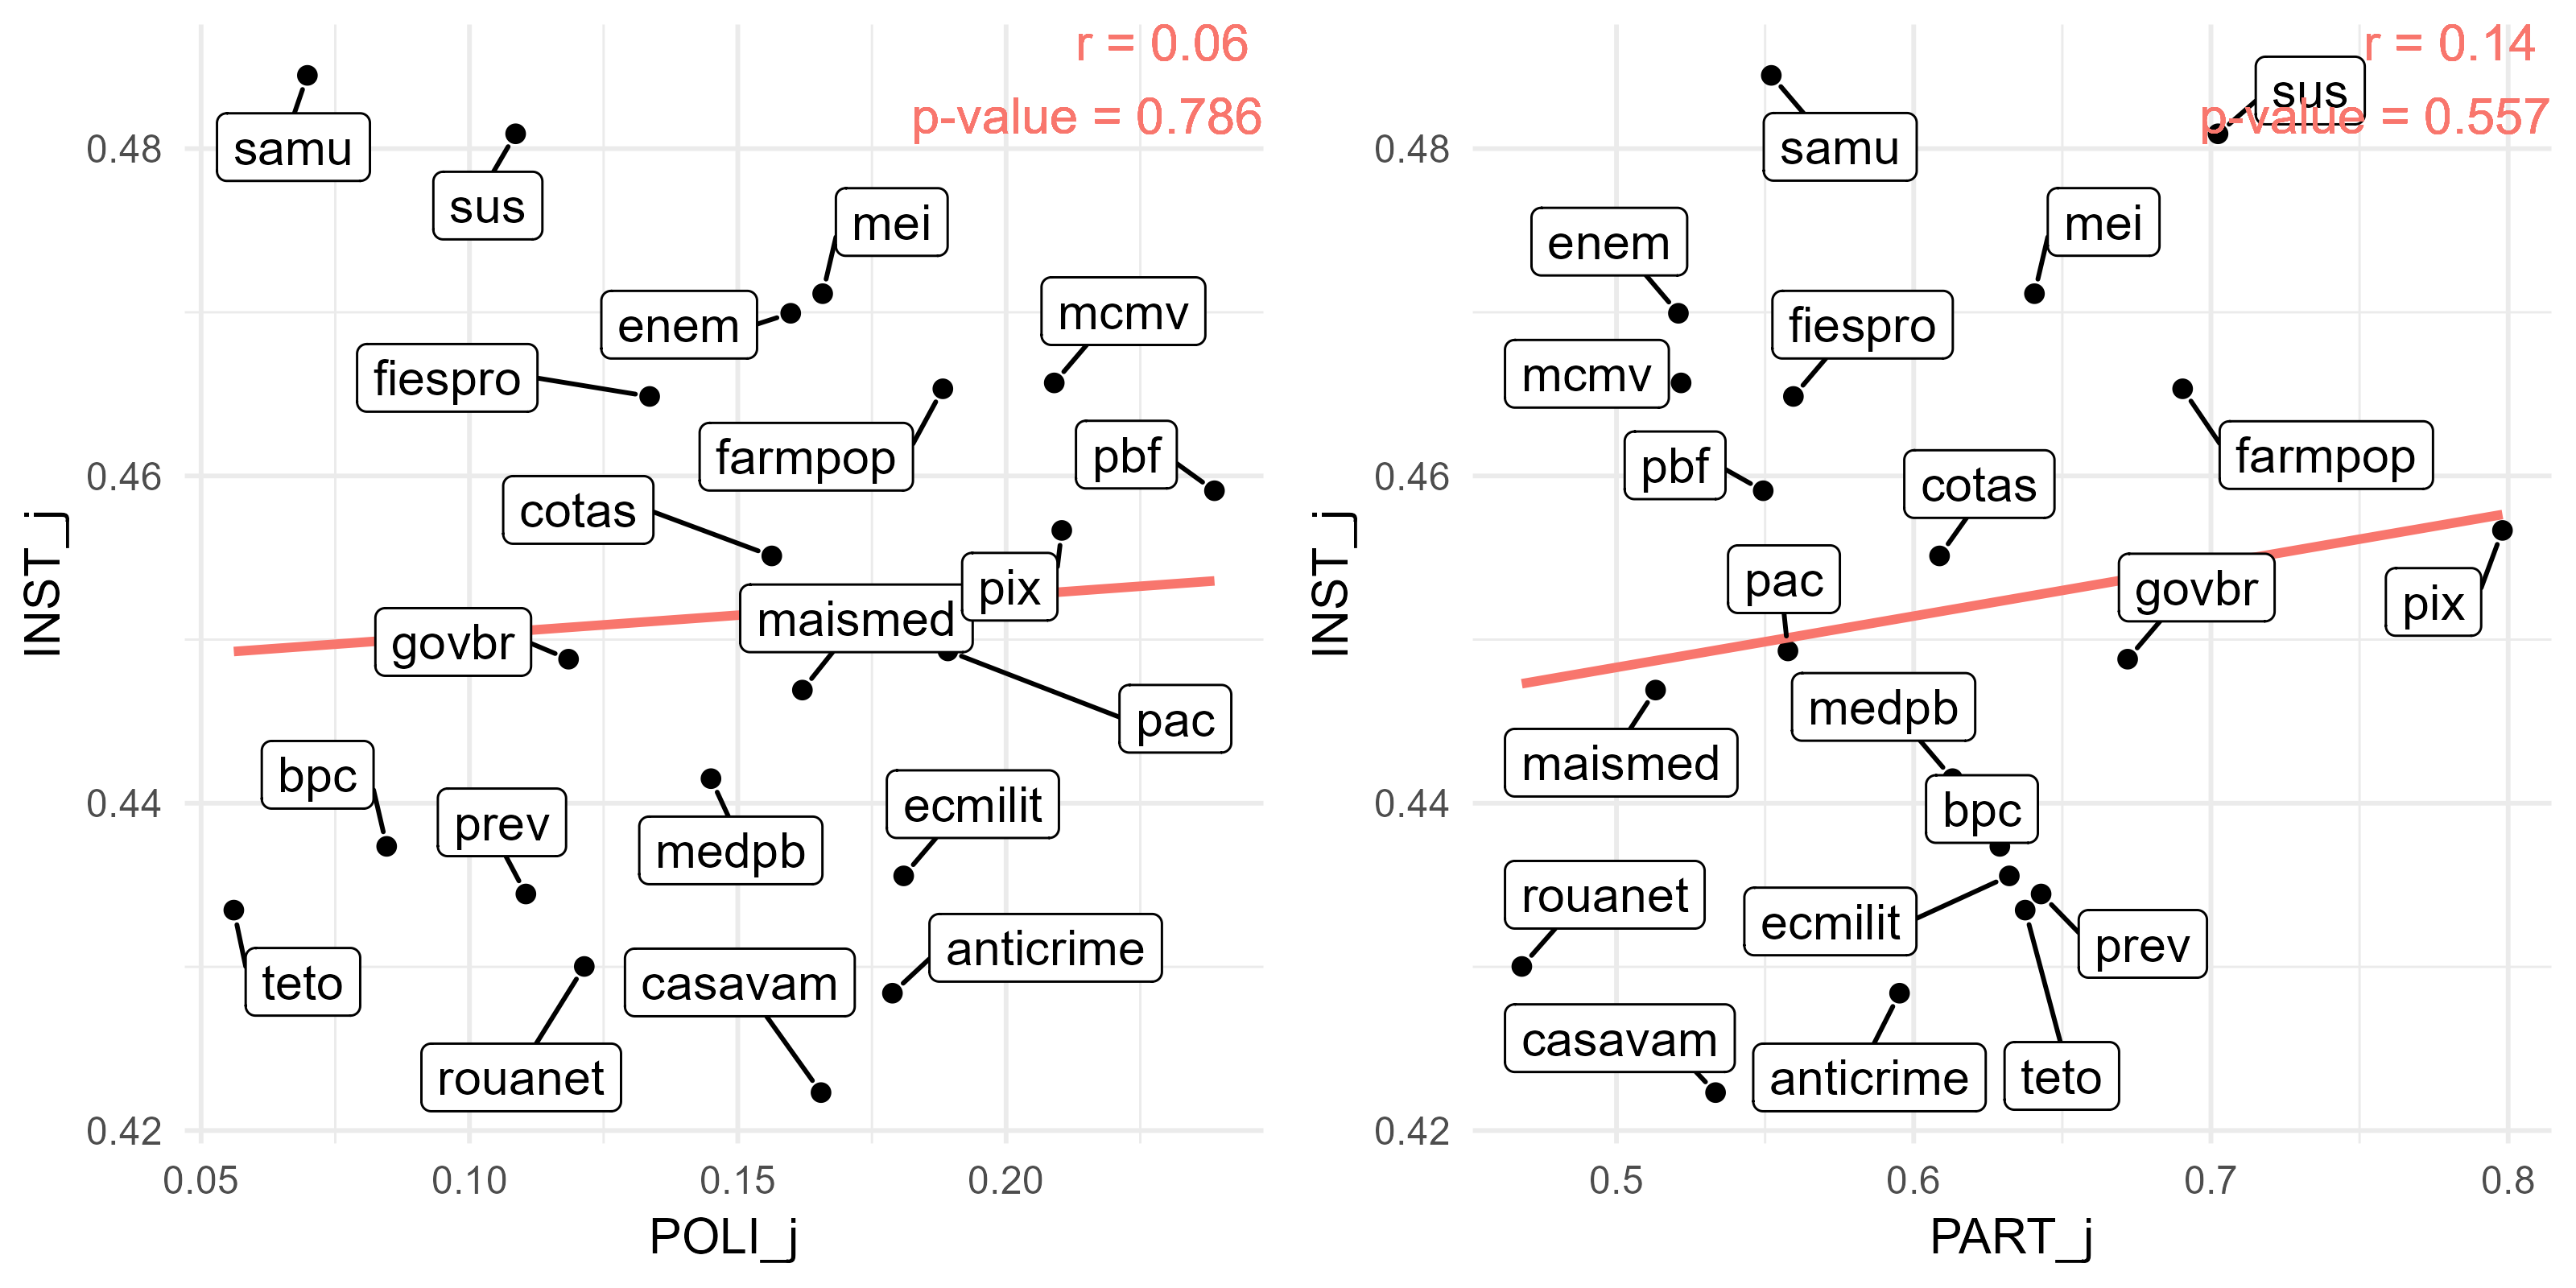
\includegraphics[width=0.5\textwidth,height=\textheight]{plots/figure_instxpolipart.png}
\caption{H1 Aggregated Test}
\end{figure}

\begin{itemize}
\tightlist
\item
  Individual-level test (H1):
\end{itemize}

\begin{enumerate}
[1)]
\tightlist
\item
  Institutionalization -\textgreater{} Policy ownership (0.14, p
  \textless{} 0.01);
\item
  Institutionalization -\textgreater{} Alignment with the owner (0.06, p
  \textgreater{} 0.05).
\end{enumerate}
\end{frame}

\begin{frame}{Study 3}
\phantomsection\label{study-3-2}
\begin{figure}
\centering
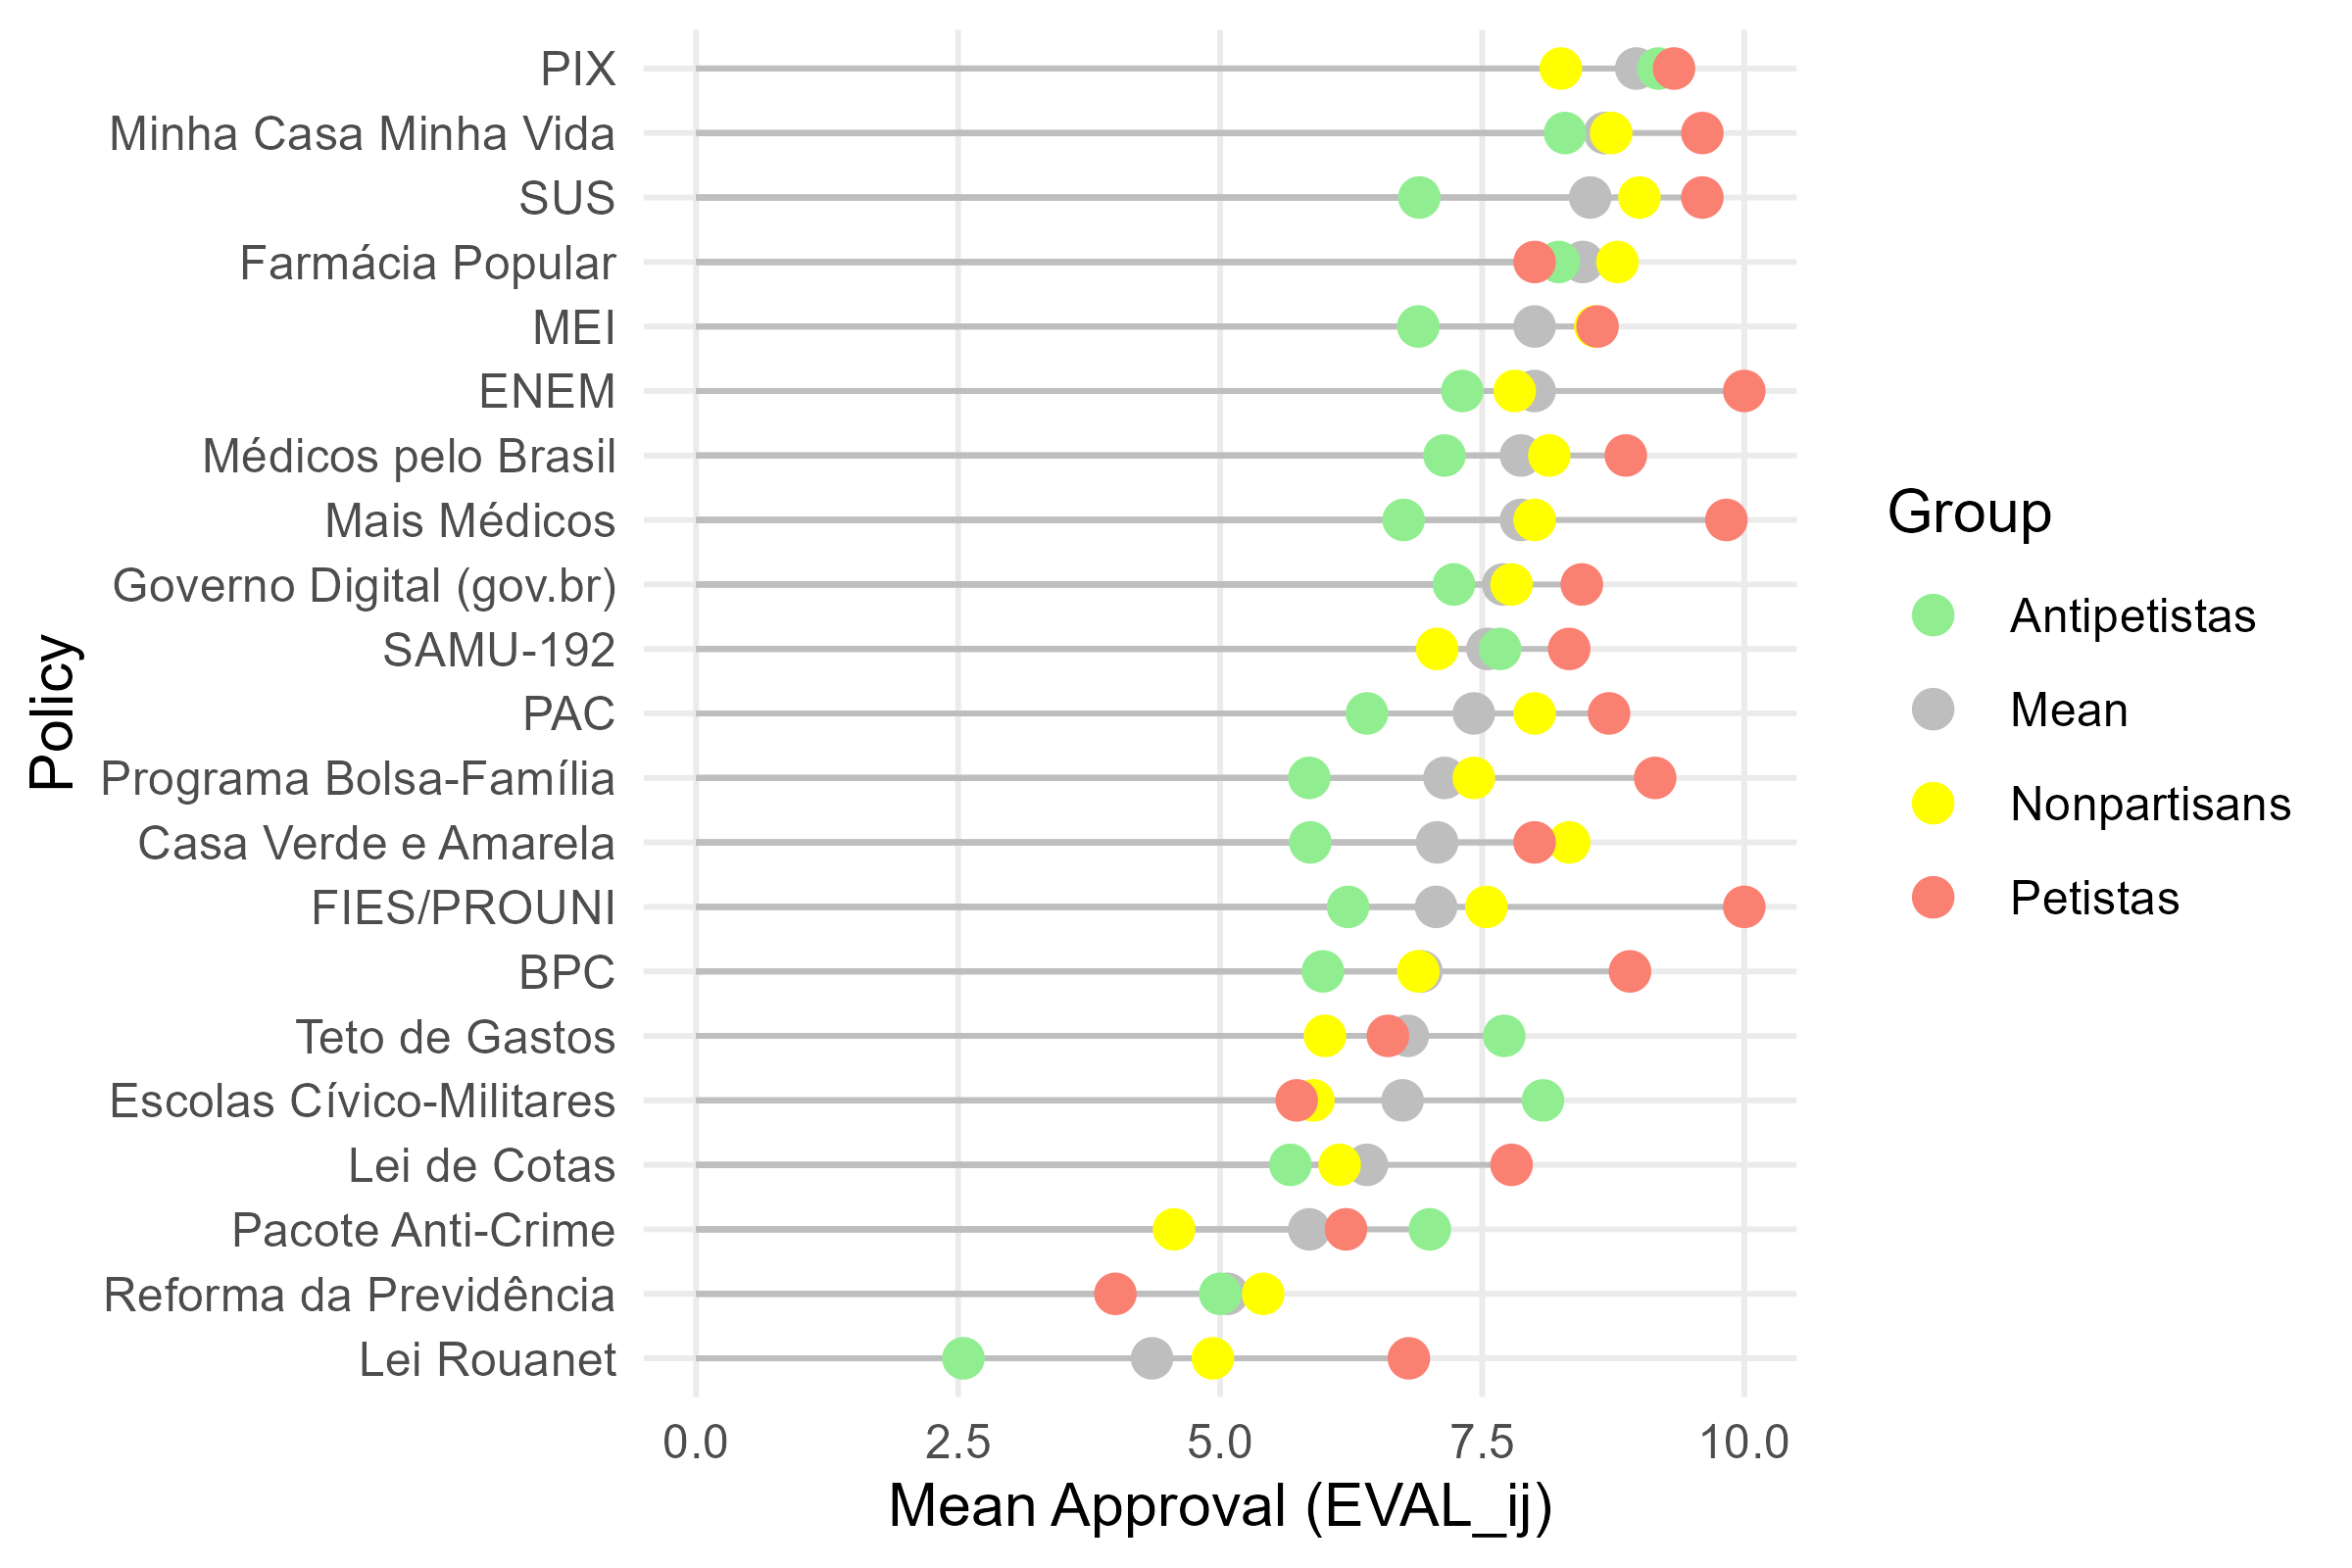
\includegraphics[width=0.55\textwidth,height=\textheight]{plots/figure_eval.png}
\caption{Approval of Policies}
\end{figure}

\begin{itemize}
\tightlist
\item
  Individual-level test (H2 and H3):
\end{itemize}

\begin{enumerate}
[1)]
\tightlist
\item
  Alignment with the owner -\textgreater{} Approval (0.40, p \textless{}
  0.001);
\item
  Policy ownership -\textgreater{} Approval (0.12, p \textless{} 0.001).
\item
  Institutionalization -\textgreater{} Approval (0.33, p \textless{}
  0.001).
\end{enumerate}
\end{frame}

\section{Conclusions}\label{conclusions}

\begin{frame}{Conclusions}
\begin{itemize}
\tightlist
\item
  Contributions:
\end{itemize}

\begin{enumerate}
[1)]
\tightlist
\item
  Methodological;
\item
  Theoretical;
\item
  Practical.
\end{enumerate}

\begin{itemize}
\tightlist
\item
  Limitations:
\end{itemize}

\begin{enumerate}
[1)]
\tightlist
\item
  Potential reverse causality;
\item
  Potential confounders;
\item
  Limited sample;
\item
  Unexplored method.
\end{enumerate}

\begin{itemize}
\tightlist
\item
  Future agenda.
\end{itemize}
\end{frame}

\section*{References}\label{references}
\addcontentsline{toc}{section}{References}

\begin{frame}[allowframebreaks]{References}
\phantomsection\label{refs}
\begin{CSLReferences}{1}{0}
\bibitem[\citeproctext]{ref-abramowitz_negative_2018}
Abramowitz, Alan I., and Steven W. Webster. 2018. {``Negative
Partisanship: Why Americans Dislike Parties but Behave Like Rabid
Partisans.''} \emph{Political Psychology} 39 (S1): 119--35.
\url{https://doi.org/10.1111/pops.12479}.

\bibitem[\citeproctext]{ref-hainmueller_causal_2014}
Hainmueller, Jens, Daniel J. Hopkins, and Teppei Yamamoto. 2014.
{``Causal {Inference} in {Conjoint Analysis}: {Understanding
Multidimensional Choices} via {Stated Preference Experiments}.''}
\emph{Political Analysis} 22 (1): 1--30.
\url{https://doi.org/10.1093/pan/mpt024}.

\bibitem[\citeproctext]{ref-kahneman_prospect_1979}
Kahneman, Daniel, and Amos Tversky. 1979. {``Prospect {Theory}: {An
Analysis} of {Decision} Under {Risk}.''} \emph{Econometrica} 47 (2):
263. \url{https://doi.org/10.2307/1914185}.

\bibitem[\citeproctext]{ref-levitsky_variation_2009}
Levitsky, Steven, and María Victoria Murillo. 2009. {``Variation in
{Institutional Strength}.''} \emph{Annual Review of Political Science}
12 (1): 115--33.
\url{https://doi.org/10.1146/annurev.polisci.11.091106.121756}.

\bibitem[\citeproctext]{ref-north_institutions_1990}
North, Douglass C. 1990. \emph{Institutions, {Institutional Change} and
{Economic Performance}}. 1st ed. Cambridge University Press.
\url{https://doi.org/10.1017/CBO9780511808678}.

\bibitem[\citeproctext]{ref-petrocik_issue_1996}
Petrocik, John R. 1996. {``Issue {Ownership} in {Presidential
Elections}, with a 1980 {Case Study}.''} \emph{American Journal of
Political Science} 40 (3): 825. \url{https://doi.org/10.2307/2111797}.

\end{CSLReferences}
\end{frame}

\end{document}
